\section{Spectre}
\label{sec:spectre}

Spectre wurde von verschiedenen Forschenden entdeckt (Project~Zero und Paul C.~Kocher + weitere) und am 3.~Januar~2018 veröffentlicht~\cite{kocher2018spectre}.
Hardwarehersteller wie Intel, AMD usw.~sowie Softwarehersteller wie Microsoft wurden bereits am 1.~Juni 2017 im Vorfeld informiert, um die Lücke bereits im Voraus durch Softwareupdates zu schließen. \\
Spectre ist ein Angriff, der Daten über einen Cache-Side-Channel ausliest.
Bei Side-Channels handelt es sich um indirekte Informationen, die über ein System gewonnen werden können, wie beispielsweise der Stromverbrauch der CPU, Elektromagnetische Strahlung, Zeitmessungen oder sogar Geräusche.
Spectre analysiert die Zugriffszeiten auf Daten, um zu bestimmen, ob diese aus dem Arbeitsspeicher geladen werden mussten (Zugriff dauert mehrere 100 Zyklen) oder durch vorherige Zugriffe bereits in den Cache geladen wurden (Zugriff dauert <10 Zyklen).
Um diese Daten in den Cache zu laden, nutzt Spectre die spekulative Ausführung von Befehlen, um Daten zu laden, die normalerweise nicht geladen werden dürften.
Die spekulative Ausführung erlaubt das Laden dieser Daten, da die Überprüfung, ob der Zugriff auf diese Daten überhaupt legitim ist, erst zur \enquote{tatsächlichen} und nicht spekulativen Ausführung erfolgt.

\subsection{Vorgehensweise}
\label{subsec:vorgehensweise}%
\begin{itemize}
    \item \textbf{1. Schritt:} 2 Arrays mit verschiedenen Größen (\texttt{array1: 16 Elemente, array2: 265 * 512 Elemente}) werden allokiert, die später für spekulative Zugriffe und Cache-Messungen verwendet werden.
    \item \textbf{2. Schritt:} Es wird berechnet, wie weit der auszulesende Speicherbereich vom Anfang von \texttt{array1} entfernt ist.
    Dieser Abstand wird benötigt, um einen Index zu bestimmen, der beim Zugriff auf \texttt{array1} tatsächlich auf den Zielbereich verweist.
\end{itemize}

\noindent
\begin{minipage}{0.58\textwidth}
    \begin{itemize}
        \item \textbf{2. Schritt:} Spectre nutzt folgenden Code, um den Cache zu trainieren: \\
        \texttt{array2[array1[x] * 512]} \\
        Dieser Aufruf nutzt den Wert, der sich in array1 an der Stelle x befindet (multipliziert mit 512), um auf einen Wert in array2 zuzugreifen.
        Der Wert, welcher sich tatsächlich in array2 befindet, ist hier irrelevant.
        Ein solcher Aufruf mit dem Wert \texttt{x=2} hätte zur Folge, dass der Wert an der Stelle \texttt{array2[array[2] * 512]} in den Cache geladen wird.
        Befindet sich an der Stelle \texttt{array1[2]} der Wert \texttt{4} der Teil des \texttt{arrays2} and der Stelle \texttt{array2[4 * 512]} in den Cache geladen.
    \end{itemize}
\end{minipage}%
\hfill%
\begin{minipage}{0.4\textwidth}
    \centering
    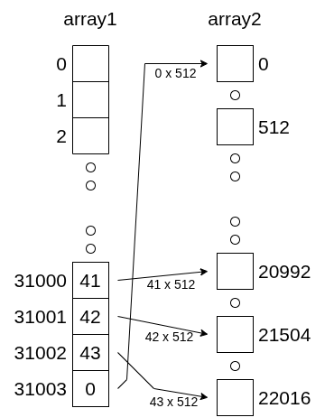
\includegraphics[width=\linewidth]{Attack-2} % replace with actual file name
\end{minipage}


\begin{itemize}
    \item \textbf{3. Schritt:} Die oben genannte Zeile wird mehrmals in einer Schleife ausgeführt, um den Branch Predictor zu trainieren.
    Hierbei werden \texttt{x} Werte verwendet, die innerhalb des \texttt{arrays1} liegen.
    Dies lässt die CPU vermuten, dass zukünftige Durchläufe der Schleife ebenfalls diesen Aufruf ausführen werden, was wiederum zur Folge hat, dass für zukünftige \texttt{x} Werte der Aufruf bereits spekulativ ausgeführt wird.
    \item \textbf{4. Schritt:} Der Wert \texttt{x} wird auf einen Wert gesetzt, der sich nicht im \texttt{array1} befindet.
    Dieser Wert entspricht dem Abstand zwischen dem \texttt{array1} und einem Bereich im Arbeitsspeicher, der versucht wird mit diesem Exploit auszulesen.
    Die CPU führt durch das vorherige Training den spekulativen Zugriff auf \texttt{array1} aus, obwohl der Wert \texttt{x} nicht im \texttt{array1} vorhanden ist.
    Beispielsweise könnte \texttt{x=2000} gesetzt werden, was zur Folge hat, dass der Wert, der sich in \texttt{array1} an der Stelle \texttt{2000} befinden würde, geladen wird (In C entspricht der Zugriff mit \texttt{array[x]} der Startadresse von \texttt{array} + \texttt{x} * Größe des Datentyps).
    Da \texttt{array1} aber nur 16 Elemente lang ist, befinden sich an dieser Stelle andere Werte (die wir spekulativ auslesen wollen).
    Der Wert, welcher sich an dieser Stelle befindet, der sich im Bereich von 0 bis 255 befindet, wird nun mit dem Wert \texttt{512} multipliziert und genutzt, um auf ein Element in \texttt{array2} zuzugreifen.
    Dieser Zugriff hat für uns zwar keinen direkten Nutzen, da sich in \texttt{array2} keine interessanten Werte befinden, führt aber dazu, dass der Teil dieses Arrays, auf den soeben zugegriffen wurde, in den Cache geladen wird.
    (Die Abstände von 512 Bytes sind so groß gewählt und zu verhindern, dass mehrere Teile des \texttt{array2} in den Cache geladen werden.)
    \item \textbf{5. Schritt:} Durch eine spezielle Bedingung wird verhindert, dass der Zugriff auf \texttt{array1} tatsächlich ausgeführt wird, um einen Segmentation Fault zu verhindern.
    Dies sorgt dafür, dass die ausgeführt spekulative Ausführung des Zugriffs auf \texttt{array1} verworfen wird und es somit auch nicht mehr möglich ist, den Wert, der sich an dieser Stelle befunden hat, im weiteren Verlauf des Programms zu verwenden.
    \item \textbf{6. Schritt:} Nun werden alle 255 möglichen Werte, die sich an der Stelle \texttt{array1[x]} befinden könnten, nacheinander getestet.
    Hierfür wird gemessen wie lange ein Zugriff auf das Element \texttt{array2[i * 512]} dauert.
    Falls sich an der Stelle \texttt{array1[x]} z.B.~der Wert \texttt{4} befunden hat, würde dies bedeuten, dass die spekulative Ausführung das Element \texttt{array2[4 * 512]} in den Cache geladen hat.
    Wird nun gemessen, dass der Zugriff auf \texttt{array2[4 * 512]} deutlich schneller ist als der Zugriff auf andere Elemente wie \texttt{array2[0 * 512]} oder \texttt{array2[5 * 512]} so kann davon ausgegangen werden, dass sich an der Stelle \texttt{array1[x]} der Wert \texttt{4} befunden hat.
\end{itemize}